\subsection{}
A monopoly market is the opposite of a perfectly competitive market.\\
A monopoly has 5 assumptions or characteristics.
\begin{enumerate}
    \item The firm is a price maker.
    \item Many buyers and one seller.
    \item Heterogeneous product. The product is unique.
    \item Barriers to entry and exit. Firms cannot enter or exit the market freely.
    (i.e. entry: ownership of a resource, high startup costs, economies of scale, predatory pricing, the government itself,
    exit: government doesn't allow monopolist to leave)
    \item (Im)perfect information.
\end{enumerate}
Examples of monopolies are Canada Post, train and metro systems.\\
Price discriminating monopolies and single price monopolies are the two types of monopolies.\\
Price discriminating examples include student discounts on the metro.\\
For a single price monopoly, the market graph is the same as the individual firm.
The demand curve is equal to the average revenue curve.\\
The marginal revenue curve is twice as steep as the demand curve, when the demand curve is linear.\\
The market will produce where marginal cost equals marginal revenue.\\
The average cost is where the quantity produced intersects the average cost curve.\\
The profit is the area between the average cost curve and the demand curve.\\
The break even point in a monopoly is NOT the minimum of the average cost curve.\\
Monopolies can profit, loss or break even but cannot shut down.\\
In the long run, it is possible for a monopoly to make a profit or a loss.\\
The price charged by a monopoly is higher than the price charged if it were a perfectly competitive market.
\begin{figure}[H]
    \centering
    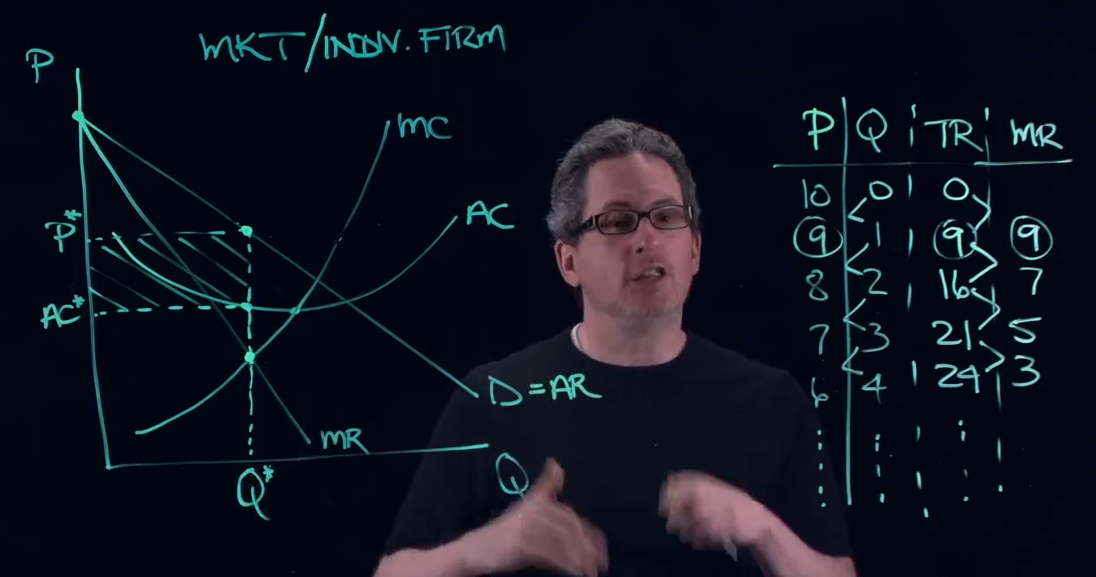
\includegraphics[width=0.5\textwidth]{Chapter10/MonopolyGraph.png}
    \caption{Monopoly Market}
    \label{fig:monopoly}
\end{figure}